\documentclass{article}
\usepackage{graphicx}
\usepackage{geometry}
\geometry{a4paper, top=2cm, bottom=2cm, left=1.5cm, right=1.5cm}
\graphicspath{{Images/}}
\usepackage{amsthm}


\begin{document}
\newtheorem{definizione}{Definizione}

\tableofcontents
\section{Tokamak}
\subsection{Struttura}
Il Tokamak si basa su tre gruppi elettromagnetici:\begin{itemize}
    \item campo toroidale: funge da manicotto e confina il plasma;
    \item magneti centrale che appartendono al trasformatore e incuono corrente nel plasma che fluisce torodialmente;
    \item magneti del campo verticale: agiscono in modo da stabilizzare il plasma e vincolarlo al centro del toro.
\end{itemize}
\subsection{Confinamento}
Per far avvenire la scarica di plasma, il tokamak deve raggiungere la cosiddetta configurazione di confinamento in cui la risultante del campo magnetico toroidale e poloidale è un campo magnetizo elicoidale: le particelle di plasma si avvitano toroidalmente in superfici isobare di flusso.
\subsection{Scarica}
Durante l'avviamento di un esperimento nel tokamak si inizia crea il vuoto all'interno del vessel e si inietta una miscela di deuterio e trizio all'interno nella camera da vuoto. A questo punto, si innalza il campo toroidale, si ha un ramp up del flusso nel trasformatore per ottenere un alto campo elettrico per poi essere interrotto. Così facendo si crea una differenza di potenziale che avvia un breakdown del plasma: gli elettroni, accelerati dal campo elettrico, guadagnano energia. Questi quando urtano gli atomi di deuterio e trizio lo possono ionizzare e generare un nuovo elettrone. Questo fenomeno si ripete esponenzialmente (avalanche) così da giungere al breakdown del plasma.\newline
Una volta che è trascorso il breakdown viene aviato il controllo in feedback del plasma.
\section{Ruolo delle misure magnetiche}
Le misure magnetiche si possono dividere in due macrocategorie:
\begin{itemize}
    \item \textbf{Operazioni real time}:\begin{enumerate}
        \item \textbf{Posizione del plasma e controllo di forma};
        \item \textbf{Sistema di protezione};
        \item \textbf{Misurazioni};
    \end{enumerate}
    \item \textbf{Analisi offline}:
    \begin{enumerate}
        \item Ricostruzioni magnetiche: superfici di flusso e il bordo del plasma. Sono molto impoortanti per correggere e interpretare le informazioni contenuta in una scarica;
        \item Analisi MHD
    \end{enumerate}
\end{itemize}
\section{Sensori Induttivi}
Il tokamak possiede delle diagnostiche basate su sensori induttivi: sono dei sensori che risentono delle variazioni del campo magnetico in forma integrale o derivativa.\\
I sensori induttivi si basano sulla legge di Faraday: la forza elettromotiva indozza è proporzionale alla derivata del flusso di campo magnetico.\begin{equation}
    fem=-\frac{d \Phi\langle B\rangle }{dt}
\end{equation}
Tuttavia in pratica quello che lo strumento ritorna sono valori di tensione che tramite la relazione:
\begin{equation}
    V=-NA\langle \dot{B}\rangle 
\end{equation}
Integrando nel tempo si può avere una misuare del flusso del campo magnetico:\begin{equation}
    \Phi=NA\langle B\rangle =-\int Vdt+const
\end{equation}
Di seguito si illustreranno i sensori induttivi installati in un tokamak.
\subsection{Rogowski Coil}
Le bobine Rogowski sono delle bobine solenoidali che si avvolgono lungo la sezione poloidale del toro. Queste forniscono una misura diretta della corrente che fluisce nel suo centro.\newline L'equazione che la caratterizza è:\begin{equation}
    \Phi = nA \oint B dl \mu_{0}nAI_p=-\int V dt+const
\end{equation}
Bisogna ricordare che:
\begin{itemize}
    \item Le misure di corrente non dipendono sulla forma del rogowski ne dalla distribuzione di corrente nel plasma;
    \item Il cammino degli avvolgimenti del solenoide devono ritornare sullo stesso asse in cui sono iniziate;
    \item Le bobine Rogowski possono essere sostituite da un set di bobine tangenti alla camera.
\end{itemize}
\subsection{Voltage Loop / Flux Loop}
Il Voltage Loop è una singolo cavo che avvolge la camera toroidalmente ed ha il compito di misurare la tensione indotta dal trasformatore centrale. La tensione ai capi della bobina vengono inviato ad un DAS che ne calcola il valore.
\subsection{Pick-Up Coils}
Le Pick-up Coils sono bobine poste al bordo del vessel utilizzare per ricostruisce l'equilibrio, per controllare il plasma e rilevare le instabilità MHD.% chktex 13
\subsection{Saddle Coils}
Le bobine Saddle sono bobine estese montate sulla camera da vuora che permettono di misuare il flusso magnetico perpendicolare a loro stessi. Inoltre, sono utilizzate per la ricostruzione dell'equilibrio e possono fornire in totale misure del flusso poloidale. In quest'ultimo caso, si ottengono misure integrali del flusso poloidale che devono essere derivare con un flusso di riferimento per ottenere una informazione.
\subsection{Loop Diamagnetico}
Sappiamo che il plasma, dall'equazione dell'equilibrio \(j\times B=\nabla p\) le particelle del plasma si dispongono lungo superficie isobare e che l'equilibrio sviluppa delle correnti poloidali che riducono il campo magnetico. Questo specifico comportamento viene detto \textbf{diamagnetismo}.\\
Al fine di misurare l'energia del plasma dal flusso toroidale si utilizza il Loop Diamagnetico. Questa misura risulta non semplice dato che l'effetto diamagnetico è molto piccolo.\newline
Infine, risulta una diagnostica che soffre dell'allineamento.
\subsection{Sensori di Hall}
Una delle problematiche delle diagnostiche a bobine magnetiche è che le misurazioni del campo magnetico rispondono a cambiamenti della derivata del campo magnetico. Ciò implica che in un campo magnetico stazionario queste bobine risultano inutili finché non vengono mosse all'interno del campo.\newline
Per questi tipi di campi si è deciso di introdurre delle diagnostiche che si basasserò sull'effetto Hall.\newline
L'effetto Hall è un fenomeno fisico proprio del plasma in cui si considera il plasma come un semiconduttore solido. In particolare, una lastra di semiconduttore è immersa in un campo magnetico. Una corrente attraversa la lastra e viene affetta dalla forza di Lorentz, deviando perpendicolarmente al prodotto vettoriare tra j e B.\newline
La carica risultante sulle facce della lastra genera un campo elettrico addizionale che cancella la forza magnetica. Quest'ultimo campo elettrico viene misurato dai sensori.
\section{Sistemi di riscaldamento addizionali}
Il principale meccanismo utilizzato nel tokamak per accellerare le particelle è il riscaldamento ohmico. Tuttavia, non è necessario ad accellerare le particelle quanto dovuto dato che questo tipo di risaldamento risulta inefficace ad alte temperature. Questo difetto è dovuto alla resistitività del plasma che diminuisce con l'aumentare della temperatura.\newline
Si necessitano di riscaldamenti addizionali per raggiungere le temperature necessarie. Esse sono basate su riscaldamento da particelle \(\alpha\), su onde elettromagnetiche e su iniezione di particelle neutre.
\subsection{Diagnostiche su atomi neutri}
Le diagnostiche basate su atomi neutri nel plasma sono importanti per plasmi confinati elettromagneticamente poiché essi, essendo neutri, attraversano le linee di campo. Possono essere quindi sfruttati per ottenere delle informazioni sul centro del plasma.\newline
Per creare un fascio neutro si utilizza una miscela da cui si producono gli ioni di deuterio o idrogeno (per maggiore efficienza si sono scelti ioni negativi), a questo punto vengono accellarati da un campo magnetico orizzontale, vengono neutralizzati e poi iniettati all'interno del plasma. Le linee guida per l'iniezione di un fascio neutro sono i seguenti:\begin{itemize}
    \item Le particelle neutre viaggiano inalterate attraverso i campi magnetici;
    \item Il beam trasferisce energia al plasma attraverso le collisioni;
    \item L'assorbimento del fascio deve avvenire al centro del plasma. Se abbiamo fomato un fascio debole allora verrà assorbito nel bordo del plasma; se troppo forte o mal direzionato può bucare la camera da vuoto;
    \item L'assorbimento del fascio dipende dalla sezione d'urto tra il fascio e il plasma;
\end{itemize}
Schematicamente:
\begin{figure}
    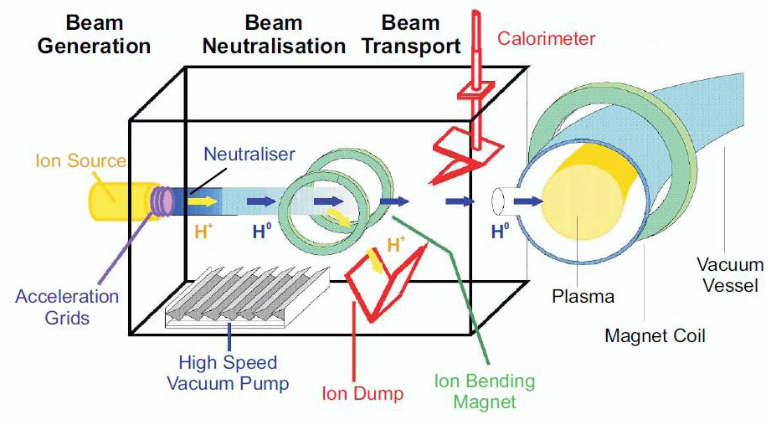
\includegraphics[scale=0.4]{2022-05-17-22-03-45.png}% chktex 8
\end{figure}
\subsection{Electron Cyclotron Resonant Heating}
Le cosiddette ECRH sono riscaldamenti addizionali basati su onde radio per trasferire energia da una sorgente esterna al plasma. Quando una onda elettromagnetica si propaga attraverso il plasma, il campo elettrico dell'onda accellera le particella cariche e quindi aumenta il numero di collisioni di queste nel plasma.\newline
In particolare, si ha assorbimento dell'onda quando si è in risonanza, tuttavia essendo il plasma non uniforme si possono avere anche fenomeni di riflessioni. Ne risulta quindi che la polarizzazione dell'onda gioca un ruolo molto importante sulla forza dell'onda e sulla regione di assorbimento. Vi sono principalmente due distinzioni di polarizzazioni che sono dipendenti dal campo magnetico nel plasma:\begin{itemize}
    \item O-Mode: parallelo al campo magnetico e inconrano solamente una frequenza di risonanza e un di cut-off;
    \item X-Mode: perpendicolare al campo magnetico
\end{itemize}
Un altro fenomeno che potrebbe risentire il fascio è quello della rifrazione quando si trannano plasmi di alta densità.
\section{Thomson Scattering}
Per misurare la temperature e la densità del plasma si sfrutta il fenomeno del Thomson Scattering. In particolare si inietta nel plasma un fascio laser e se ne misura sia la luce diffusa che la larghezza spettrale.\newline
Le misure di larghezza fornisco delle informazioni sulla temperatura e l'intensità della luce diffusa sulla densità degli elettroni. Le ragioni principali per cui si è introdotta questa diagnostica sono due:\begin{itemize}
    \item è un metodo che non perturba l'equilibrio del plasma poiché si richiede solo l'accesso alle radiazioni del plasma;
    \item permette di avere delle informazioni dettagliate sulla funzione di distribuzione degli elettroni.
\end{itemize}
Si ha una onda elettromagnetica incidente su una particella che viene accelerata dai campi elettromagnetici dell'onda. Durante l'urto si ha una emissione di una radiazione detta scattered wave. Questa radiazione viene misurata dagli spettrometri a filtri policromatrici.
Dato che occorre che il posizionamento delle ottiche sia ottimale, la calibrazione diventa fondamentale per ottenere misurazioni della densità di elettroni. Essa viene effettuata utilizzando altri gas.
\section{Polarimetro}
Il polarimetro è necessario per ottenere informazioni sulla densità e corrente di plasma. Si basa principalmente su due fenomeni:\begin{itemize}
    \item Effetto Faraday: nel plasma in presenza del campo magnetico, il piano di polarizzazione del fascio laser propagato nel campo magnetico ruota. Da informazioni su \textbf{Campo magnetico Poloidale};
    \item Effetto Cotton-Mouton: se il fascio laser si propaga perpendicolarmente al campo magnetico vi è un campo dell'ellitticità della polarizzazione.Da informazioni su \textbf{Campo magnetico toroidale}.
\end{itemize}
Il plasma nel campo magnetico si comporta come un mezzo dielettrico con indici di rifrazione diverse in base alle componenti del campo magnetico. In particolare, il pasma è birifrangente e questa proprietà dipende da:\begin{itemize}
    \item Densità elettronica;
    \item Il campo magnetico;
    \item Temperatura elettronica.
\end{itemize}
\begin{definizione}
    Un'onda è detta polarizzata linearmente se la risultante del campo elettrico vibra nella stessa direzione in un particolare punto.
\end{definizione}
La polarizzazione può essere ottenuta da:\begin{itemize}
    \item assorbimento selettivo;
    \item Riflessione;
    \item Scattering;
\end{itemize}
\subsection{Assorbimento Selettivo}
Nell'assorbimento selettivo, un fascio non polarizzato attraversa una lente di polarizzazione che fa passare solo le componenti del campo magnetico su un asse. Poi queste componenti incidono su un analizzatore: il raggio incidente con quello rifratto formerà un angolo che viene misurato.
La particolarità del polarizzatore è che assorbe i vettori di campo elettrico nelle direzioni perpendicolari e trasmette quelle nella direzione parallela.
\subsection{Polarizzazione da doppia rifrazione}
Esistono materiali che possiedono due inidici di rifrazioe differenti. Questi materiali vengono detto birifrangenti.\\
Ne è un esempio la calcite che, quando la luce non polarizzata attraversa il materiale viene divisa in due: raggio straordinario E (varia in base alla direzione di propagazione) e raggio ordinario O (è la stessa lungo tutte le direzioni). Inoltre, vi è una direzione detta \textbf{asse ottico}, su quale i raggi ordinari e straordinari hanno la stessa velocità.
\subsection{Funzionamento}
Supponiamo di avere una onda luminosa che si propaga lungo la direzione z. Sappiamo che questa è una onda elettromagnetica con le componenti del campo magnetico e elettrico perpendicolari l'una dall'altra. Tramite delle funzioni trigonometriche e passaggi algebriche si arriva allìequazione di una ellisse. Quando questo raggio luminoso attraversa il plasma si nota che l'ellisse viene ruotata di un certo angolo
\section{Interferometro}
\section{MSE}
\section{Neutronica}
\section{Disruzioni}
Le disruzioni nei Tokamak sono inevitabili. Esse sono una perdita globale di confinamento e controllo del plasma dovuto da impurezze e radiazioni.\newline
Si compongono di due fasi:
\begin{itemize}
    \item Termal quence: perdita di tutta l'energia cinetica e termica;
    \item Current quence: decadimento di corrente
\end{itemize}
In particolare, si ha una fase lontana dalla disruzione non si ha un indizio della disruzione. Dopo di che, si ha un segnale di precorso nelle bobine magnetiche che indica l'inizio di una anomalia. Passata questa fase, si hanno delle anomalie sul profilo di temperatura e corrente così da innescare il termal quence e quindi l'inizio di una disruzione, perdendo di conseguenza il controllo.\newline
Il problema principale di questo fenomeno è che avvenuta la disruzione si danneggiano i dispositivi e si introducono impurezze nel vessel che diminuiscono il tempo operativo del Tokamak. I danni principali sono:
\begin{itemize}
    \item Carichi termici;
    \item Estinzione della corrente rapida porta a carichi magnetici molto elevati dovuto alle correnti indotte (Eddy current);
    \item Elettroni di runaway nella fase di current quenche: in questa fase il plasma perde la densità, così vengono accellarati notevolmente divenendo un fascio di elettroni incontrollato in assenza di collisioni per limitarne la velocità.
\end{itemize}
\subsection{Classificazione diagnostiche disruzione}
L'obiettivo delle diagnostiche per le disruzioni è quello di predizioni, spiegazione e controllo. Si dividono in:
\begin{itemize}
    \item monitorazione delle conseguenze;
    \item misura della disruzione;
    \item investigazione della fisica della disruzione;
    \item predizione delle disruzione
\end{itemize}
Queste diagnostiche fanno parte del sistema di controllo e quindi è necessario che l'hardware siano affidabili, disponibili, forniscano un risoluzione spaziale e temporale per prevenire il fenomeno e devono coprire tutti i punti della camera da vuoto. Inoltre, al livello di processamento deve essere in real-time ed avere capacità predittive.
Una scarica disruttiva presenta la seguente nomenclatura:
\begin{itemize}
    \item Avoidance: la fase lontana di disruzione;
    \item Prevenzione: azione correttiva per evitare l'instabilità;
    \item Mitigazione: nel caso in cui la prevenzione non è abbastanza d avviene la disruzione si riducono i carichi abbassando lentamente la corrente e l'energia termica. In questo fase possono avvenire i run-away. Si immettono pellet di gas per ridurre il carico termico o degli shattered pellet.
\end{itemize}
\subsection{Requisiti Hardware}
\subsubsection{Carichi termici}
Il problema principale sono i carichi termici che dipendono dalla potenza deposita, dalla superfice e dal tempo. Le misure che si utilizzano sono:\begin{itemize}
    \item Camere termiche;
    \item Spettrometria;
    \item Bolometria
\end{itemize}
La problematica di queste misure è che il carico termico non sono toroidalmente simmetrici.
\subsubsection{Carichi Meccanici}
Le misure che si utilizza sono:\begin{itemize}
    \item bobine in posizioni differenti per eseguire una ricostruzione dell'equilibrio;
    \item Misure delle correnti toroidali del vessel (Halo currents);
    \item Accelerometria per misurare gli spostamenti della camera da vuoto
\end{itemize}
\subsection{Locked mode detection AUG}
Siamo nella fase di mitigazioni per cui dobbiamo predirre con un margine di predizioni basso, ma molto accurato.\newline
In questa fase, vi sono delle instabilità MHD macroscopiche con misure magnetiche grande. La crescita delle istabilità vengono misurate con la componente radiale del campo magnetico tramite le Saddle Coils. In un tokamak ve ne sono 4 e tramite la differenza di queste bobine opposte e tramite un indicatore si misura l'effetto di rallentamento delle instabilità. Esse crescono nella fase preliminare della disruzioni, poi rallentano fino a zero e poi disrompe. Viene detto bloccato poiché il campo magnetico da loro generato si blocca con gli errori del Tokamak divenendo stazionari nel sistema di riferimento del laboratorio.\newline
Analizzando lo spettro a bassa frequenza si nota che le instabilità MHD non sono le uniche fautrici delle disruzioni, ma anche dovute dai cosiddetti ELMS.% chktex 13
\subsection{Imaging for disruptions}
Si utilizzano delle telecamere nel visibile per avere una idea di quello che accade nella camera da vuoto. Risulta quindi molto importante cercare di ricoprire il maggiorspazio dellla camera da vuoto e del vessel. Tramite queste telecamere è possibile rivelare i MARFE.\newline
I MARFE sono instabilità termiche che si manifestano come un anello di radiazioni visibili per effetto delle impurezze. In queste zone la temperatura risulta più bassa rispetto al plasma.
\subsection{Indicatori di Profilo}
Per la predizione delle disruzione e il controllo in feedback sono necessari gli indicatori di profilo.\\ GLi indicatori di profilo per la predizione devono essere robusti e calcolabili in real time, ma allo stesso tempo devono fornire  un quantitativo sufficiente di informazioni. Uno degli indicatori sul profilo di temperatura è la hollowness cioè quanto il profilo di temperatura è cavo. Questa è una misura particolarmente difficile da quantificare dato che in molti casi si deve effettuare il mirroring dei dati sull'asse magnetico per un problema di coverage e che è resiliente sulle fluttuazioni della temperatura.\newline
Per questa misura si utilizza un fitting basato su due Gaussiane quando il profilo è cavo: differenze tra i due massimi e normalizzata per la deviazione standard delle  gaussiane. Con questo approccio, più due massimi sono distanti più il profilo sarà cavo.
\subsection{Problema inverso nella fusione}
Per quanto riguardo le misure effettuate dall'esterno del plasma, esse vengono utilizzate nella risoluzione di un problema inverso per ottenere delle informazioni dell'interno. Il principale strumento che viene utilizzato è la tomografia.
\end{document}